\subsubsection{UC6.3 - Personalizzazione Force Field}
\begin{figure}[h]
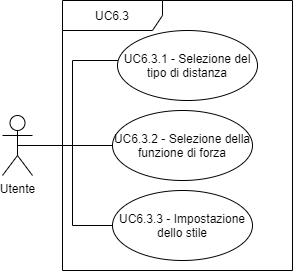
\includegraphics[width=9cm]{../Images/UC6.3.png}
\centering
\caption{UC6.3 - Personalizzazione Force Field}
\end{figure}
\begin{itemize}
	\item \textbf{Attore primario}: Utente.
	
	\item \textbf{Precondizioni}: L'utente ha scelto il grafico \textit{Force Field} [UC5.3].
	
	\item \textbf{Postcondizioni}: Il grafico viene aggiornato.
	
	\item \textbf{Scenario principale}: L'utente decide:
	
\begin{enumerate}
\item Il tipo di distanza per il calcolo [UC6.3.1];
\item Il tipo di funzione di forza [UC6.3.2];
\item Alcuni stili del grafico [UC6.3.3].
\end{enumerate}	
		
\end{itemize}

